%% Chapter 6 - Results

\chapter{Results}
\label{ch:results}

\section{Quantitative Results}
\label{sec:results-quant}

The strongest quantitative result obtained in the current phase is the binary
bone-loss classifier, which achieved a validation macro-F1 of 0.9233 on the
held-out Tufts validation split. The overlap-based severity classifier and the
caries severity stage are weaker but still useful intermediate baselines,
whereas the CEJ branch remains exploratory.

\begin{table}[htbp]
  \centering
  \caption{Validated results currently supported by saved artifacts.}
  \label{tab:results-comparison}
  \begin{tabular}{@{}lcccc@{}}
    \toprule
    Module & Accuracy & Key class recall & Specific note & Macro-F1 \\
    \midrule
    Bone-loss binary & -- & 0.8305 & Specificity = 0.9953 & 0.9233 \\
    Bone-loss severity & -- & -- & Mild F1 = 0.80 & 0.7208 \\
    Caries severity (initial phase 2) & 0.80 & Deep-caries recall = 0.59 & Preserved notebook output & 0.73 \\
    Caries severity (best preserved phase 2) & 0.81 & Deep-caries recall = 0.84 & Final refined run & 0.77 \\
    \bottomrule
  \end{tabular}
\end{table}

The quantitative evidence for the caries branch requires one clarification. The
exported collaborator notebook preserves the validation reports for the second
stage of the cascade (caries versus deep caries), but the final printed report
for the first-stage caries versus no-caries classifier is not present in the
checked notebook artifact. Therefore, Table~\ref{tab:results-comparison}
reports only the validated caries-stage outputs that can be directly recovered
from the repository.

\begin{figure}[!htbp]
  \centering
  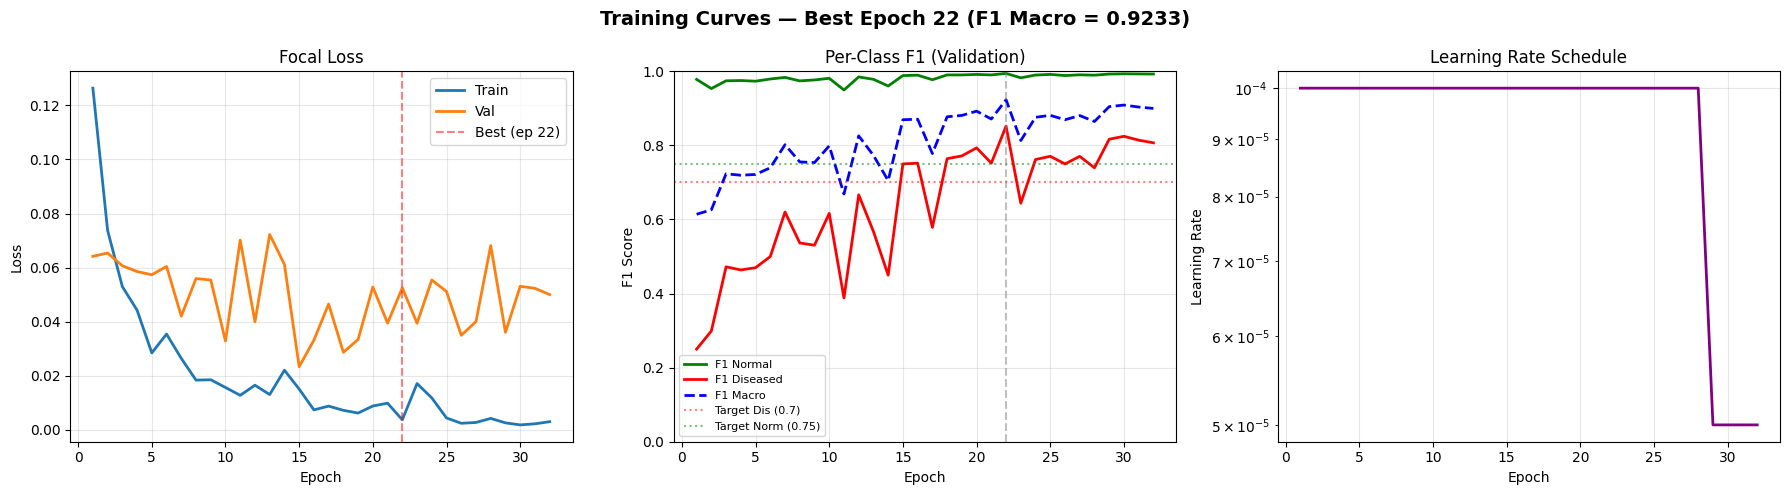
\includegraphics[width=0.82\linewidth]{figures/bone_loss_training_curves.png}
  \caption{Training and validation curves for the binary bone-loss classifier.}
  \label{fig:bone-loss-training-curves}
\end{figure}

Figure~\ref{fig:bone-loss-training-curves} shows stable optimization behavior
for the binary periodontal model. The best checkpoint was selected from the
validation trajectory, not simply from the final epoch.

\begin{table}[htbp]
  \centering
  \caption{Detailed periodontal branch results.}
  \label{tab:periodontal-results}
  \begin{tabular}{@{}lccc@{}}
    \toprule
    Metric & Binary bone loss & Severity classifier & CEJ v2 \\
    \midrule
    Validation set size & 1,558 & positive subset & 296 crops \\
    Sensitivity / recall & 0.8305 & -- & reliable on 62.5\% \\
    Specificity & 0.9953 & -- & -- \\
    Macro-F1 & 0.9233 & 0.7208 & -- \\
    Exact agreement with overlap labels & -- & -- & 15.1\% \\
    Agreement within \(\pm 1\) class & -- & -- & 61.6\% \\
    \bottomrule
  \end{tabular}
\end{table}

\begin{figure}[!htbp]
  \centering
  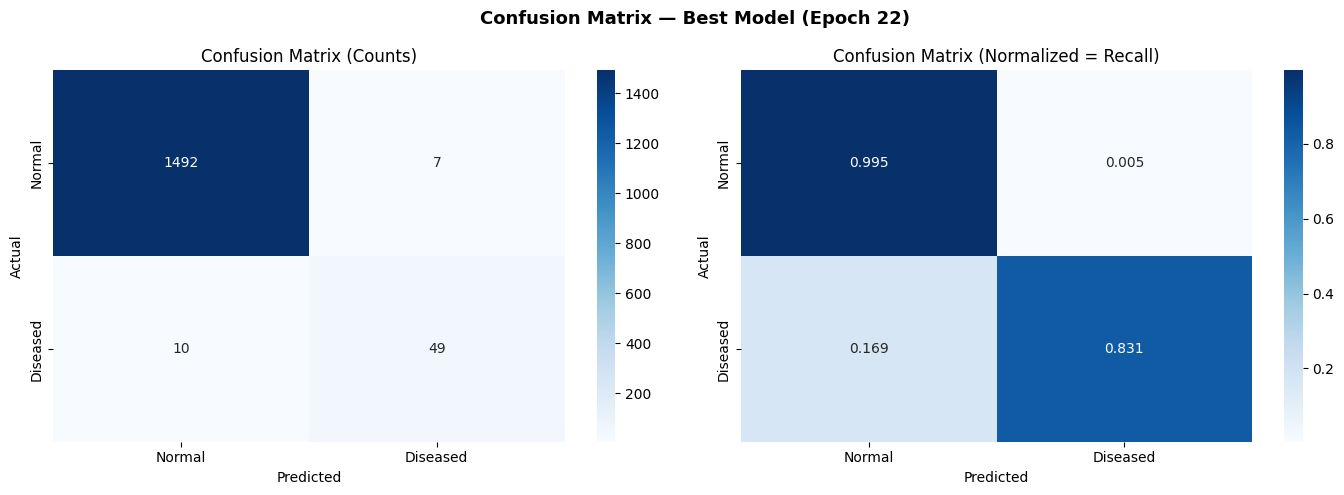
\includegraphics[width=0.58\linewidth]{figures/bone_loss_confusion_matrix.png}
  \caption{Confusion matrix of the binary bone-loss classifier on the validation split.}
  \label{fig:bone-loss-cm}
\end{figure}

Figure~\ref{fig:bone-loss-cm} highlights the strongest property of the binary
model: very low false-positive rate with still useful diseased-case recall.

\section{Qualitative Results}
\label{sec:results-qual}

Two qualitative observations are consistent across the experiments. First, the
binary periodontal classifier is robust on clearly normal and clearly diseased
crops, which suggests that the asymmetric crop design successfully exposes the
relevant bone context to the network. Second, the failure cases cluster around
more ambiguous boundaries: mild versus moderate bone loss, and caries versus
deep caries. This is expected because both tasks depend on relatively small
visual differences within a limited dataset.

The CEJ branch provides the clearest failure analysis. It can usually locate a
candidate landmark pattern after CLAHE preprocessing, but overlapping
structures, metallic restorations, and anterior-tooth morphology variations
often make the measurement clinically unreliable. This is precisely why the CEJ
branch is not used as the primary severity output despite being conceptually
closer to the periodontal gold standard.

\begin{figure}[!htbp]
  \centering
  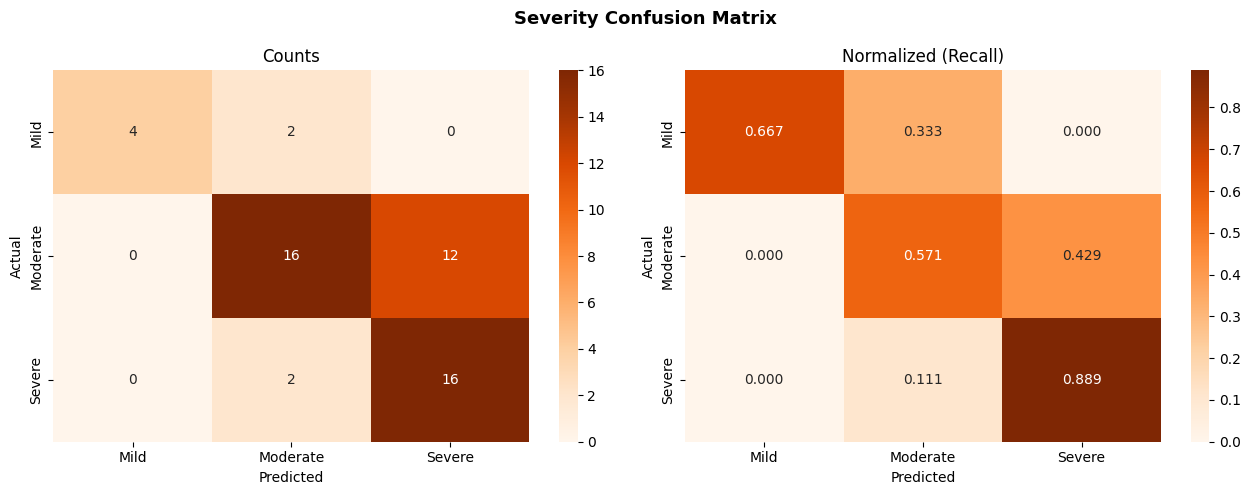
\includegraphics[width=0.58\linewidth]{figures/bone_loss_severity_confusion_matrix.png}
  \caption{Confusion matrix for the overlap-based three-class bone-loss severity model.}
  \label{fig:bone-loss-severity-cm}
\end{figure}

Figure~\ref{fig:bone-loss-severity-cm} shows that severity staging is harder
than binary detection. Most errors occur between adjacent severity categories,
which is clinically more plausible than random confusion.

% Suggested figures for the final camera-ready version:
% 1. Bone-loss crop with expert mask overlay and predicted class.
% 2. CEJ v2 success case with detected landmarks and confidence score.
% 3. CEJ v2 failure case showing why the heuristic is unreliable on some OPGs.
% 4. Caries severity examples: caries vs deep-caries confusion pair.

\section{Ablation / Comparative Analysis}
\label{sec:results-ablation}

Although a formal ablation table is not yet available for every branch, three
comparative findings are already supported by the current artifacts.
\begin{enumerate}
  \item Correct annotation parsing mattered more than model complexity.
  Fixing the Tufts \texttt{External ID} join bug and the bounding-box coordinate bug
  was essential; without these fixes, the periodontal pipeline would have been
  trained on mismatched labels and incorrect crops.
  \item Overlap-based severity is currently more practical than CEJ-based
  severity on panoramic OPGs. The CEJ branch is clinically attractive, but its
  agreement with overlap-derived labels remains too weak to use as the primary
  severity estimator.
  \item The caries cascade benefited from low-learning-rate refinement in
  phase 2. The preserved results improved from macro-F1 0.72 to 0.77 and
  deep-caries recall from 0.78 to 0.84 after reweighting and additional
  fine-tuning.
\end{enumerate}

\begin{figure}[!htbp]
  \centering
  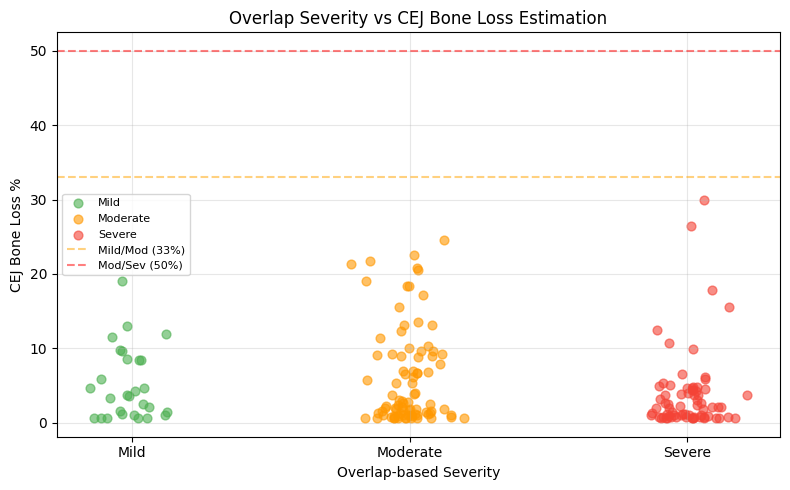
\includegraphics[width=0.62\linewidth]{figures/cej_agreement_analysis.png}
  \caption{Agreement analysis between CEJ-based estimation and overlap-based severity labels.}
  \label{fig:cej-agreement}
\end{figure}

Figure~\ref{fig:cej-agreement} supports the decision to retain CEJ as an
exploratory branch. The current agreement is informative, but not strong enough
for primary severity reporting on panoramic OPGs.

\section{Discussion}
\label{sec:results-discussion}

The main result of this phase is that the periodontal branch is not merely an
idea but an implemented and quantitatively validated subsystem. A standard
ResNet18, when paired with correct tooth-level crop construction and imbalance
handling, is already strong enough to detect bone loss reliably on the held-out
Tufts validation set. This is the clearest technical success in the repository.

The limitations are equally important. The overall project is still modular
rather than integrated; there is no full-OPG inference script yet. The caries
branch depends on notebook artifacts with incomplete experiment logging for the
first-stage metrics. The CEJ branch remains exploratory, and no calibrated
confidence layer or Grad-CAM reporting layer has been integrated into the final
workflow. These gaps define the next phase of work rather than weakening the
value of the completed modules.
